\subsection{MinSort}

\begin{frame}{MinSort - Algorithm}
  \begin{columns}
    \begin{column}{0.5\textwidth}
      \textbf{Informal description:}
      \begin{itemize}
        \item
          Find the minimum and switch the value with the
          {\color{Mittel-Blau}first} position
        \item
          Find the minimum and switch the value with the
          {\color{Mittel-Blau}second} position
        \item
          $\cdots$
      \end{itemize}
    \end{column}
    \begin{column}{0.5\textwidth}
      \begin{figure}[!h]%
        \begin{adjustbox}{width=\linewidth}
          \begin{adjustbox}{width=\linewidth}
\begin{tikzpicture}[
  swap/.style={
    draw,
    line width=0.4em,
    color=Mittel-Blau
  }
]
\foreach[count=\x] \h/\c in {
  1/Hell-Gruen,%
  2/Hell-Gruen,%
  3/Hell-Gruen,%
  12/Hell-Blau,%
  7/Hell-Blau,%
  4/Mittel-Blau,%
  6/Hell-Blau,%
  10/Hell-Blau,%
  8/Hell-Blau,%
  15/Hell-Blau,%
  14/Hell-Blau,%
  5/Hell-Blau,%
  11/Hell-Blau,%
  9/Hell-Blau,%
  13/Hell-Blau%
} {
\draw[fill=\c] (\x + 0.1, 0.0) rectangle (\x + 0.9, \h/2);
\draw (\x + 0.5, -0.5) node {\huge \h};
}

\draw[swap, <->] (4.5, 6.5) to [out=90,in=90,looseness=2] (6.5, 2.5);
\draw (5.5, 7.75) node[label={\Huge swap}] {};
\end{tikzpicture}
\end{adjustbox}%
        \end{adjustbox}
        \caption{\textit{MinSort} at the fourth iteration}%
        \label{fig:minsort_fourth_iteration}%
      \end{figure}%
    \end{column}
  \end{columns}
\end{frame}

%-------------------------------------------------------------------------------

\codeslide{python}{
\begin{frame}{MinSort - Algorithm}
  \textbf{MinSort in Python:}
  \lstinputlisting[
    language=Python,
    style={python-idle-code},
    basicstyle=\small,
    tabsize=4,
    emph={minsort},
    emphstyle=\color{blue}
  ]{Code/MinSort/MinSort.py}
\end{frame}
}

\codeslide{java}{
\begin{frame}{MinSort - Algorithm}
  \textbf{MinSort in Java:}
  \lstinputlisting[
    language=Java,
    style={java-eclipse-code},
    basicstyle=\small,
    tabsize=4,
    emph={minSort},
    emphstyle=\color{blue}
  ]{Code/MinSort/MinSort.java}
\end{frame}
}

\codeslide{cpp}{
\begin{frame}{MinSort - Algorithm}
  \textbf{MinSort in C++:}
  \lstinputlisting[
    language=C++,
    style={cpp-eclipse-code},
    basicstyle=\small,
    tabsize=4,
    morekeywords={size_t},
    emph={min_sort},
    emphstyle=\color{blue}
  ]{Code/MinSort/MinSort.cpp}
\end{frame}
}

%-------------------------------------------------------------------------------

\begin{frame}{MinSort - Runtime}
  \textbf{How long does our program run?}\vspace*{-0.5em}
  \begin{columns}%
    \begin{column}{0.415\textwidth}
      \begin{itemize}
        \item
          We test it for different input sizes
        \item
          \textbf{Observation:}\\
          It is going to be \enquote{disproportional}
          slower the more numbers are being sorted
      \end{itemize}
    \end{column}%
    \begin{column}{0.585\textwidth}%
      \vspace*{-1.0em}%
      \begin{table}[!h]%
        \caption{Runtime for \textit{MinSort}}%
        \label{tab:minsort_runtime}%
        \begin{tabular}{c|c}%
          $n$ & Runtime / \si{\milli\second}\\
          \midrule
          \num{2e3} & \num{5.24}\\
          \num{4e3} & \num{16.92}\\
          \num{6e3} & \num{39.11}\\
          \num{8e3} & \num{67.80}\\
          \num{10e3} & \num{105.50}\\
          \num{12e3} & \num{150.38}\\
          \num{14e3} & \num{204.00}\\
          \num{16e3} & \num{265.98}\\
          \num{18e3} & \num{334.94}
        \end{tabular}
      \end{table}
    \end{column}
  \end{columns}
\end{frame}

%-------------------------------------------------------------------------------

\begin{frame}{MinSort - Runtime}
  \textbf{How long does our program run?}\vspace*{-0.5em}
  \begin{columns}
    \begin{column}{0.415\textwidth}
      \begin{itemize}
        \item
          We test it for different input sizes
        \item
          \textbf{Observation:}\\
          It is going to be \enquote{disproportional}
          slower the more numbers are being sorted
      \end{itemize}
    \end{column}
    \begin{column}{0.585\textwidth}
      \begin{center}%
        \begin{figure}%
          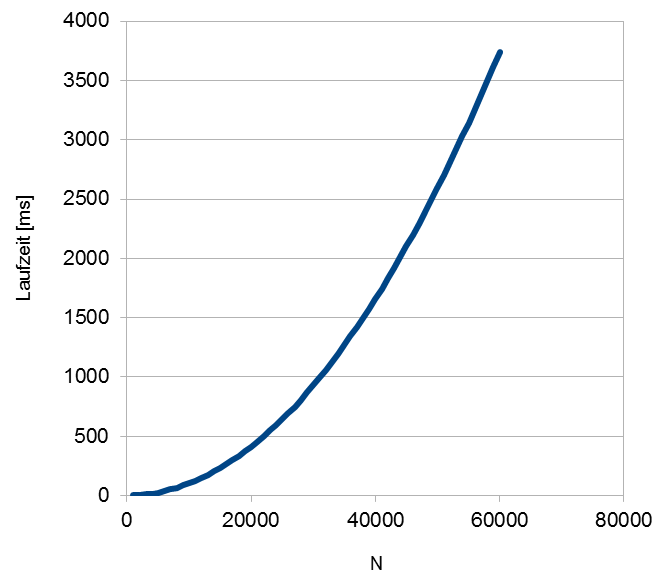
\includegraphics[width=\textwidth]{Images/MinSort/RuntimeSquared.png}%
          \vspace*{-1.0em}\caption{Runtime of \textit{MinSort}}%
          \label{fig:minsort_runtime}%
        \end{figure}%
      \end{center}
    \end{column}
  \end{columns}
\end{frame}

%-------------------------------------------------------------------------------

\begin{frame}{MinSort - Runtime}
  \begin{columns}%
    \begin{column}{0.5\textwidth}%
      \textbf{Runtime analysis:}
      \begin{itemize}
        \item
          In this lecture we study this diagram for \textit{MinSort}
          \begin{itemize}
            \item
              Thats what you should do in the first exercise sheet
          \end{itemize}
        \item
          \textbf{We observe:}\\
          \begin{itemize}
            \item
              The runtime {\color{Mittel-Blau}grows faster than linear}
            \item
              With double the input size we need four times the time
          \end{itemize}
      \end{itemize}
    \end{column}%
    \begin{column}{0.5\textwidth}%
      \begin{center}%
        \begin{figure}%
          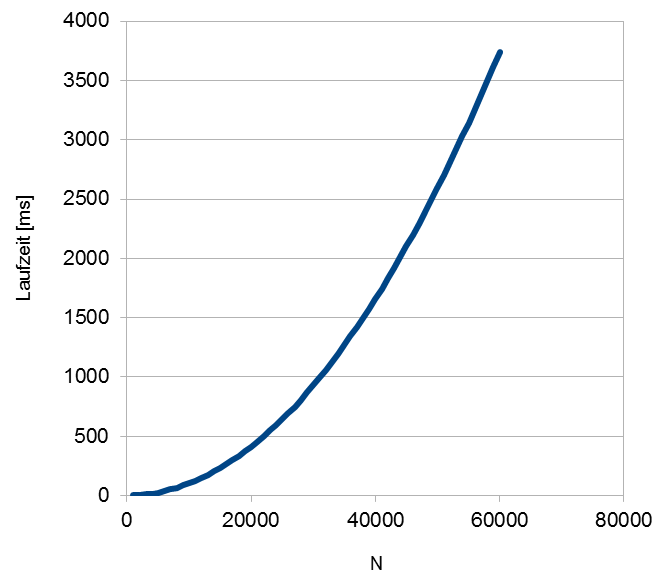
\includegraphics[width=\textwidth]{Images/MinSort/RuntimeSquared.png}%
          \vspace*{-1.0em}\caption{Runtime of \textit{MinSort}}%
          \label{fig:minsort_runtime_2}%
        \end{figure}%
      \end{center}
    \end{column}%
  \end{columns}
  \begin{columns}
    \begin{column}{1.0\textwidth}
      \begin{itemize}
        \item
          Next lecture we will analyze deeper with other methods
      \end{itemize}
    \end{column}
    % Dummy column
    \begin{column}{0.0\textwidth}\end{column}
  \end{columns}
\end{frame}